\documentclass[a4paper, 12pt]{article}
\usepackage{a4wide}
\usepackage{amsfonts} % if you want blackboard bold symbols e.g. for real numbers
\usepackage{graphicx} % if you want to include jpeg or pdf pictures
\usepackage{listings}\lstset{columns=fullflexible}
\usepackage{xspace}
\usepackage[show]{ed}
\usepackage{tikz}
\usetikzlibrary{shapes.geometric,docicon}
\usepackage{longtable}

\usepackage[hyperref=auto,style=alphabetic,isbn=false]{biblatex}
\addbibresource{kwarcpubs.bib}
\addbibresource{extpubs.bib}
\addbibresource{kwarccrossrefs.bib}
\addbibresource{extcrossrefs.bib}
\addbibresource{kat.bib}


\def\defemph#1{\textbf{#1}}

\usepackage[linkcolor=black,citecolor=black,urlcolor=black,colorlinks=true,breaklinks=true,
plainpages=false,pdfpagelabels]{hyperref}

\title{\KAT: An Annotation Tool for STEM Documents}
\author{Alex Dumitru, Deyan Ginev, Michael Kohlhase\\
  Vlad Merticariu, Stefan Mirea, Tom Wiesing\\[1ex]
Computer Science,  Jacobs University Bremen\\
\url{http://kwarc.info}}
\date{\today}
\def\KAT{\textsf{KAT}\xspace}
\begin{document}
\maketitle
\begin{abstract}
  Current natural language understanding systems do not work particularly well on
  mathematical and technical documents as they cannot deal with formulae, diagrams, and
  the special, technical vocabularies and discourse conventions of such documents. To
  retrain existing tools and evaluate new ones specifically developed for STEM documents,
  we need to establish manually annotated document corpora. Unfortunately, even the
  annotation tools used in computational linguistics do not work well with mathematical
  documents, as they assume plain texts.

  This report presents the \sys system, browser-based annotation tool for
  linguistic/semantic annotations in structured (XHTML5) documents. As it is parametric in
  the annotation ontology and represents annotations as RDF, it can easily be integrated
  into RDF-based corpus management systems; we present an integration into the CorTeX
  system.
\end{abstract}

\thispagestyle{empty} \newpage
\tableofcontents\newpage

\section{Introduction}\label{sec:intro}
Text annotation is the practice of adding a note to a text, which may include highlights
or underlining, comments, footnotes or links.  In most of the cases,annotations can be
thought of as text-metadata because they are usually added post hoc and provide
information about the text without fundamentally altering it.

A web annotation is an online annotation associated with a web resource. The annotation of
web-based documents by user communities is a widely used method of augmenting and adding
value to these resources and there are numerous use cases where the process can
disambiguate contexts or improve the overall readability.

In this report we presen the \KAT annotation tool for (X)HTML documents, built with the
following objectives:
\begin{enumerate}
\item \emph{Usability} -- The tool should be convenient and easy to use by regular
  internet users allowing them varying degrees of complexity in the user interface.
\item \emph{Ease of integration} -- The tool should be easy to integrate into existing
  projects, and should have minimal to none dependencies on the server side.
\item \emph{Semantic Richness} -- The annotations provided by our users should contain the
  necessary level of information for NLP tools to use.
\end{enumerate}
In the next section we review the state of the art, \ednote{MK: continue}

%%% Local Variables: 
%%% mode: latex
%%% TeX-master: "kat"
%%% End: 

\section{State of the art}
In this section we will present a few of the current annotation tools available on the
web, extracting the most relevant features that were taken into account when building
\KAT.

Different types of web-based projects will require different approaches to annotations,
allowing us to distinguish between 2 main categories:
\begin{enumerate}
\item \defemph{Dynamic annotations}: implemented by systems which allow the annotation of
  the text itself. In such a system, the anchor of an annotation is a piece of digitized
  text.
\item \defemph{Static annotations}: implemented by systems which allow the annotation of a
  specific region of content. In this case, the anchor of an annotation is the fixed,
  in-page, position of the annotated region.
\end{enumerate}
Digitized, mathematical text lays in the center of our research direction during this
project and, for this reason, we are going to focus mainly on the first category. However,
in order to have a complete overview of the available features, the last subsection of
this part presents one example from the second category.

An important aspect of our desired system is that, even though it is very close to a
dynamic annotation system, we are looking for a more stable and semantically rich format,
such as \textsf{OMDoc}, to anchor the annotations.

\subsection{the brat Annotation Tool}

brat~\cite{brat:on} Is a web based tool for text annotation. It is designed in particular
for structured annotation, where the notes are not freeform text but have a fixed form
that can be automatically processed and interpreted by a computer and implicitly belongs
to the category of dynamic annotation tools.
\begin{figure}[ht]\centering
 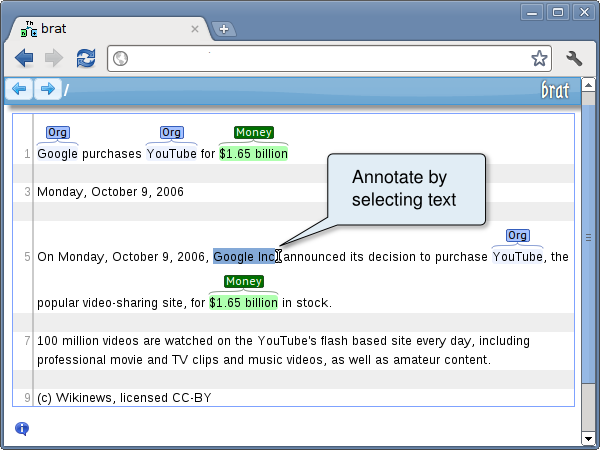
\includegraphics[width=3.7in]{figures/brat}
 \caption{Annotation with brat}\label{fig:brat}
\end{figure}
The most important features that we identified were:
\begin{enumerate}
\item The text must be preprocessed into a particular, fixed format before being
  annotated.
\item There are 2 types of annotation supported:
  \begin{itemize}
  \item text span annotations: simple annotation of a piece of text:
   \begin{center}
     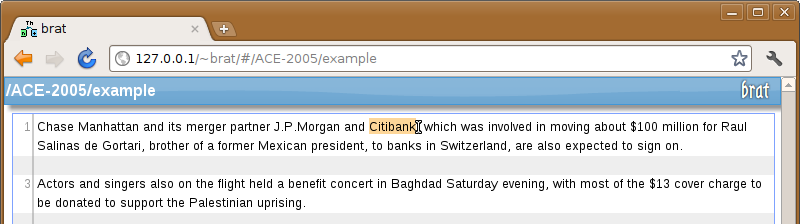
\includegraphics[width=3.5in]{figures/brat-text-span}
   \end{center}
   
  \item relation annotations: two separated pieces of text are annotated and a connection between them is created:
    \begin{center}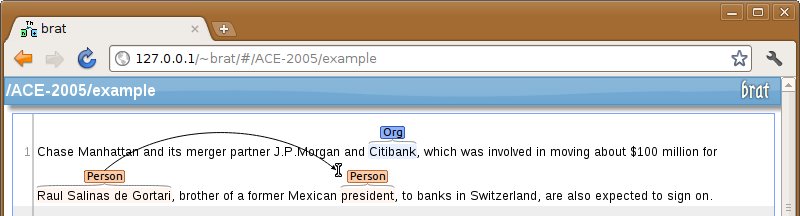
\includegraphics[width=3.5in]{figures/brat-relation}\end{center}
  \end{itemize}
\item Extensive search functionality for annotations, see Figure~\ref{fig:brat-search}
\item Export interface: annotations can be exported in an internal format, which can then
  be converted in other formats such as PDF or HTML. Furthermore, visualizations can be
  exported as well, into SVG and bitmap formats (PNG).
\item Each annotation is accessible by URL: every brat annotation can be uniquely
  addressed within the brat server. Together with the URL of the server, this form of
  addressing provides a globally unique address for every brat annotation.
\item Brat provides a validation system for its annotations: the admin can define
  validation grammar rules, forcing the user to adhere to a specific annotation format.
\item Annotations are anchored based on a word-counter: this makes the annotated text
  unchangeable and constitutes one of our main concerns regarding the system.
\end{enumerate}
\begin{figure}[ht]\centering
  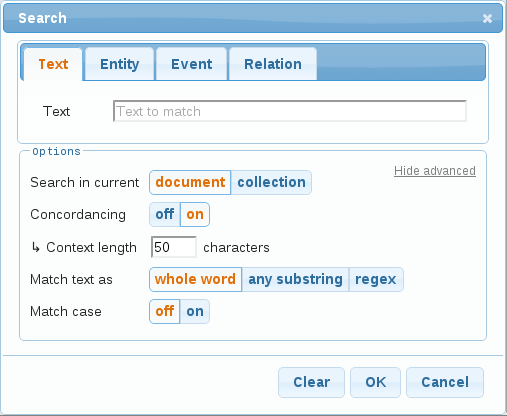
\includegraphics[width=3.5in]{figures/brat-search}
  \caption{Search in brat}\label{fig:brat-search}
\end{figure}

\subsection{Yawas Annotation Tool} 
Yawas~\cite{yawas:on} is an annotation system designed as an extension for Firefox and
Google Chrome; see Figure~\ref{fig:yawas} It is different than the other systems that we
analyzed in that the annotation doesn't belong to the text but to the user. After
installing the extension, the use can navigate to any page and can highlight any piece of
text. The annotation is saved in the user's google account and is displayed every time the
user accesses the page.

\begin{figure}[ht]\centering
  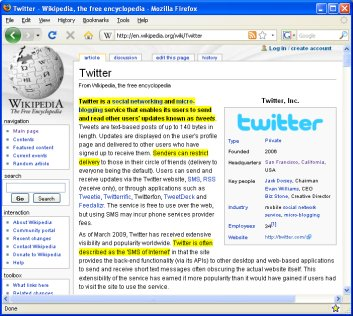
\includegraphics[width=2.5in]{figures/yawas}
  \caption{Annotation in Yawas}\label{fig:yawas}
\end{figure}

Feature-wise the system is much weaker than the previously analyzed brat (and much older),
however it contains a potentially useful idea: user-specific annotations which can later
be made accessible only to specific users or groups of users.

\subsection{Annotatie Systeem Annotation Tool} % Roman numerals
Annotatie~\cite{annotatie:on} is an annotation tool for printed
documents and belongs to the static annotation category.\vspace{10pt}

The anchoring of the annotations is done by page positioning: this seems inflexible at a
first glance, however, it constitutes a good alternative when the text in the page is not
digitized.  The feature that caught our attention is the extensive comment sectioned
derived from the annotations:
\begin{itemize}
\item Each annotation represents a new comment thread.
\item In each comment thread other users can further discuss on both the contents of the
  annotated text and the annotation itself.
\item All the annotations in a page are displayed in the right side of the page, as
  collapsed threads.
\end{itemize}
We believe that allowing discussion based on one user's annotation is an important feature
in such a system, as the context introduced by annotations is one which emphases user
collaboration.


%%% Local Variables: 
%%% mode: latex
%%% TeX-master: "kat"
%%% End: 

\section{\KAT System \& Information Architecture}\label{sec:sysarch}

\begin{figure}[ht]\centering
\begin{tikzpicture}[yscale=1.5]
\tikzstyle{doc}=[draw,align=center,color=black,shape=document]
\tikzstyle{database}=[cylinder,shape border rotate=90,aspect=0.25,draw, 
     cylinder uses custom fill,cylinder body fill=yellow!30,cylinder end fill=yellow!30]
  \pgfdeclareimage[width=1cm]{user}{user};
  \node (user) at (-1,2) {\pgfuseimage{user}};
  \node[doc] (onto) at (6,2) {\begin{tabular}{c}Annotation\\Ontology\end{tabular}};
  \node[database] (docstore) at (0,0) {\begin{tabular}{c}Document
      \\Store\\\hline tHTML5 \end{tabular}};
  \node[database] (semblack) at (5,0) {\begin{tabular}{c}Semantic
      \\Blackboard\\\hline RDF\end{tabular}};
  \node[draw,rounded corners] (kat) at (2.5,2) {\begin{tabular}{c}KAT\\Annotator \end{tabular}};
  \draw[->] (docstore) -- node[left]{import} (kat);
  \draw[<-] (kat) to[out=-65,in=155] node[left]{import} (semblack);
  \draw[->] (kat) to[out=-25,in=105] node[right,near end]{export} (semblack);
  \draw[->,dotted] (semblack) -- node[above]{references} (docstore);
  \draw[<->] (user) -- node[above] {interact} (kat);
  \draw[->] (onto) -- node[above]{read} (kat);
\end{tikzpicture}
\caption{The \KAT System Architecture}\label{fig:kat-arch}
\end{figure}

\subsection{\KAT Annotation Data Model}
The annotations that the users will provide must be well structured in order for our third
requirement to be accomplished. This assures us that the work of annotators can best be
put to use by automatic processors or computer interpreters.

A good example of a use case is a self-learning software that translates text fragments
from one language to another.  For it to function properly it needs to know the
grammatical structure of the languages and here is where annotation tools can help.  Users
can annotate predefined sentences or paragraphs and identify specific parts of speech
(e.g. a noun) that the translation tool software developers can then use as a training
material for their machine-learning product.

Our system is flexible enough for administrators to
define how annotations should be structured and what connections can be made between
different annotations.  Furthermore this flexibility is also be applicable in the
visual interfaces with which users interact. In a typical system you will have users
coming from different backgrounds with various skills and interests. We believe that this
variety should not be suppressed but rather encouraged by allowing for multiple annotation
interfaces to be presented to the user so that he can choose the best suited one for his
contributions. This feature helps projects where crowdsourcing is detrimental by making
the users comfortable with the UI and allowing them to become proficient without a steep
learning curve.

\subsection{Concept Architecture}
At the center of our system is the \textbf{annotation concept}, several of which being
described by a user-supplied ontology. The format in which the ontology should be provided
is the standard OWL model.  Each annotation concept should correspond to an OWL instance
that is a member of the annotation class to which the following elements should be added:
\begin{itemize}
\item fields - this section describes how a user can input the necessary information for
  the annotation to be valid according to its concept. The section should contain for each
  field describing the annotation concept an entry that describes how a user can populate
  this information in a form.
  
  Each child of the entry should be of the following form:
  \begin{itemize}
  \item filed - the field wrapper, all further options are children of this element. It
    has \textit{name} and \textit{type} as attributes. The \textit{type} can be one of:
    text, select, reference, radios or text area.
  \item documentation - further information about the field, to be displayed to the user.
  \item value - a default value for the field.
  \item validation - a regular expression that the user input must match.
  \item number - a field having 2 attributes: \textit{atleast} and \textit{atmost},
    indicating how many inputs of this type can the user make in the same annotation.
  \item options [only available for field type = "select"] - the options from which the
    user should choose from. Each new option is an individual element having children of
    type \textit{documentation} and \textit{value}.
  \item referencedType [only available for field type = "reference"] - indicates the
    concept name that should be referenced by this input.
  \end{itemize}
\item display - this section describes how an annotation is displayed. It consist of the
  following fields:
  \begin{itemize}
  \item template - an HTML string containing the desired display format of the annotation
    fields. Each annotation field that is mentioned between curly braces will be replaced
    by the actual value of the field.
  \item style - a list of CSS valid rules to be applied to the annotation display.
  \end{itemize}
\end{itemize}

In Appendix A2 you can find an example of an annotation ontology. It defines 2 concepts
which allow the user to annotate text as Symbols or definitions of Symbols. As you can see
in the example, the model gives us the necessary flexibility at the administrator level
while at the same time providing for a clear customizable method of displaying the
annotation form and representation for the user.

%%% Local Variables: 
%%% mode: latex
%%% TeX-master: "kat"
%%% End: 

%  LocalWords:  sysarch tikzpicture yscale tikzstyle pgfdeclareimage pgfuseimage docstore
%  LocalWords:  hline semblack kat textbf textit textit textit atleast atmost

\section{Annotation Workflows}

\subsection{Adding an annotation}

The following steps must be followed for adding a \KAT annotation:
\begin{figure}[ht]\centering
  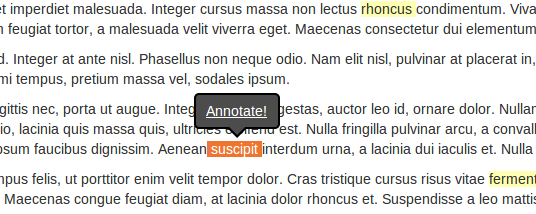
\includegraphics[width=.57\textwidth]{../PIC/annotate}\quad
  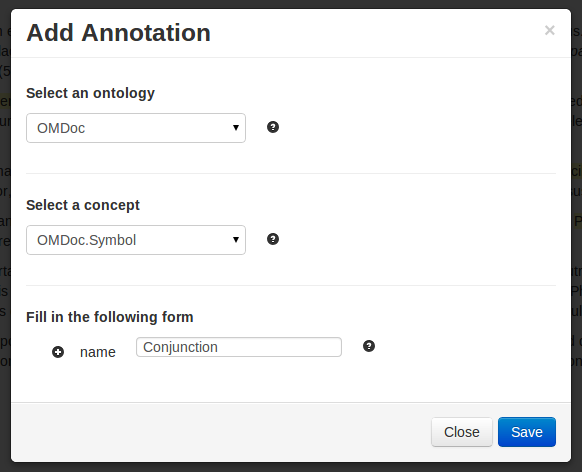
\includegraphics[width=.37\textwidth]{../PIC/add-symbol}
  \caption{Annotating in \KAT: Selection and Form-Filling}\label{fig:kat-annotate}
\end{figure}

\begin{compactenum}
\item The target text of the annotation is highlighted (by simple selection), see
  Figure~\ref{fig:kat-annotate} on the left.
\item The first step triggers an annotation-menu.
\item The annotation-menu is populated with the available annotation types, given by the
  available ontology.
\item The user clicks on the desired annotation concept.
\item A modal box containing the annotation form opens.
\item The annotation form is populated with the fields indicated in the ontology as shown
  on the right of Figure~\ref{fig:kat-annotate}
\item After completing the form fields, the user saves the annotation.
\end{compactenum}
This approach ensures 2 things:
\begin{compactitem}
\item The navigation flow is never interrupted: adding an annotation is done via pop-up
  and modal boxes and windows, so after completing the steps, the user finds himself in
  the same place in the document.
\item Annotation type checking is implicit: the annotation form is populated with the
  fields indicated in the ontology so the user doesn’t have to check the required types
  himself, see Figure~\ref{fig:kat-definition}.  In the \KAT binding, the OMDoc.Definition
  concept is defined to be for annotations of type Symbol. The ``for'' field is
  automatically populated with all the annotations of this type.
\end{compactitem}

\begin{figure}[ht]\centering
 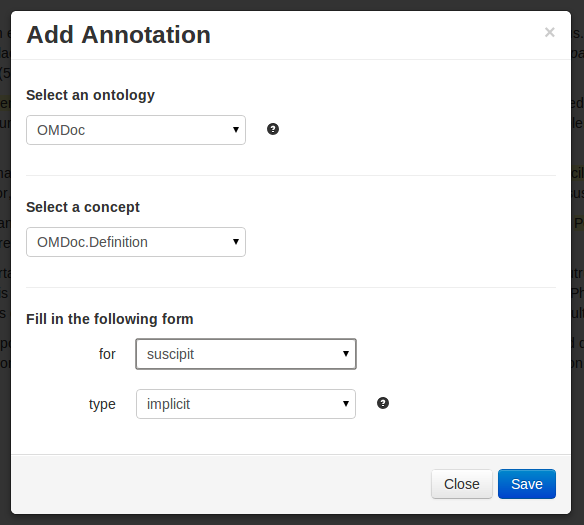
\includegraphics[width=2.5in]{../PIC/add-definition}
 \caption{Annotating a definition for ``suscipit''.}\label{fig:kat-definition}
\end{figure}

\subsection{Displaying an annotation}

Annotated text is marked with special CSS style so it becomes easily identifiable.  The
type of the annotation is also displayed above the annotation itself so one can have a
clear overview of the whole document.

At click, a pop-up window containing the annotation display opens.

The annotation display consists of the following elements:
\begin{compactenum}
\item The type of the annotation.
\item The formatted annotation input according to the rules described in the ontology.
\item For the annotations of type reference, an arrow indicated the referenced element.
\end{compactenum}

\begin{figure}[ht]\centering
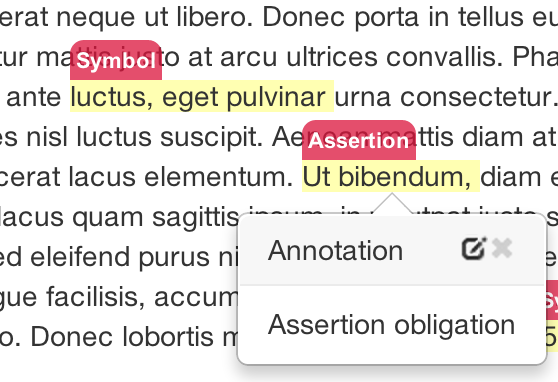
\includegraphics[width=.4\textwidth]{../PIC/suscipit}\quad
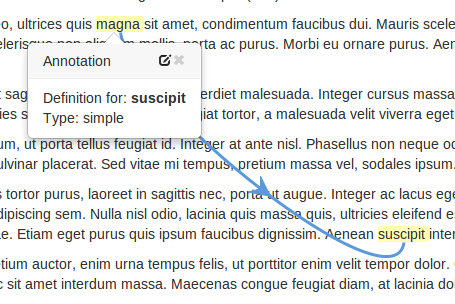
\includegraphics[width=.5\textwidth]{../PIC/definition}
\caption{Display for simple text and reference annotations}\label{fig:suscipit-definition}
\end{figure}

\subsection{Reviewing annotation versions}
\ednote{MK: need intro here, inter-annotator agreement, riew, ... Probably move into a
  section of its own.}

Reviewing is done in a side-by-side view which allows the user to see two versions of the
same document in order to see discrepancies and correct them; see
Figure~\ref{fig:kat-review}. The viewer allows to toggle view one ontology at a time which
can be toggled individually on each panel by clicking on the.

While reviewing, the left panel (also called the main panel) is the current document with
the local annotations while the right panel (referred to as the mirror panel) is the the
different version of the document being reviewed against.

\KAT is only enabled in the main panel so changes/edits/annotations can still be done
while reviewing, while the mirror panel is read-only. Scrolling the main panel will cause
the mirror panel to automatically follow suite.

\begin{figure}[ht]\centering
 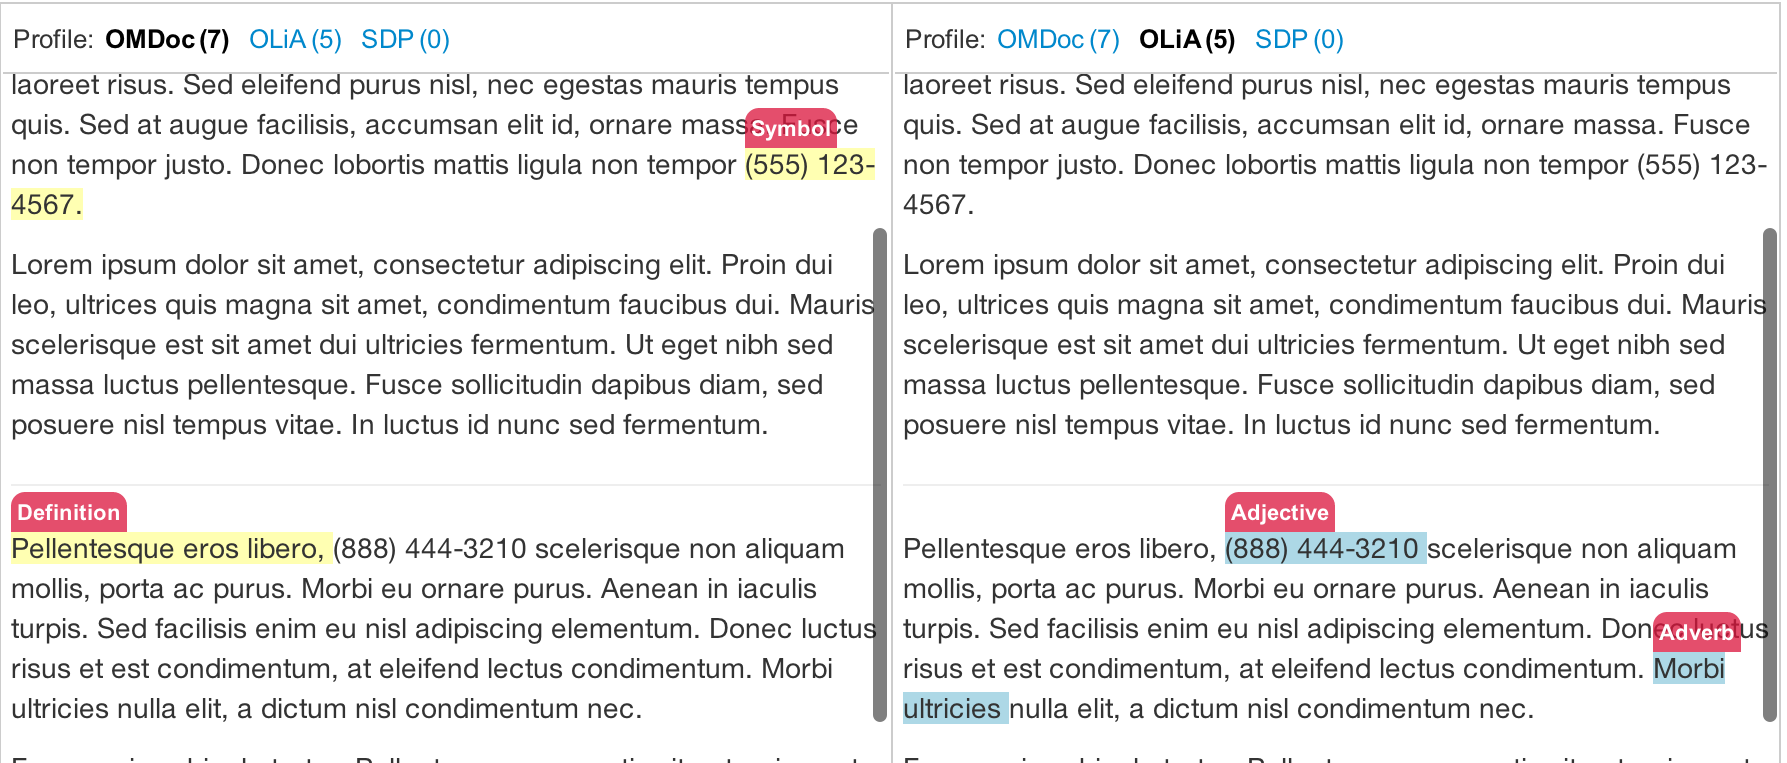
\includegraphics[width=5in]{../PIC/review}
 \caption{Reviewing two ontologies of the same document side-by-side}\label{fig:kat-review}
\end{figure}

\subsection{Annotating external documents using the browser extension}

A different way of annotating a document which is not part of the corpus is by
using the KAT browser extension. It provides a point-and-click interface which
allows users to easily select the tags they wish to annotate.


\begin{wrapfigure}l{1.5cm}\vspace*{-1em}
  
\includegraphics[width=1.5cm]{../PIC/extension-browser-icon-none}
\end{wrapfigure}
The following steps must be followed to add an annotation with the KAT browser extension.
Make sure you have the extension installed. You should see the KAT icon near your URL bar.
Under the icon the extension always displays if the page currently viewed has any
annotations or not. The figure on the right shows the \KAT browser icon when viewing a
page with no annotations on it.

\begin{wrapfigure}r{2.5cm}\vspace*{-1em}
  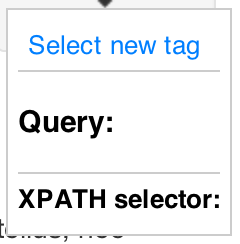
\includegraphics[width=2.4cm]{../PIC/extension-menu}
\end{wrapfigure}
After loading the page you want to annotate, click the extension icon which will insert a
menu in the page. From the menu, choose "Select new tag" as shown on the left.  When
moving your mouse around the page, the current tag is always highlighted and its
respective DOM and XPATH selectors are displayed in the menu.
After right clicking on the desired element, the "Annotate" pop-up will appear and the
current element will remain selected (see Figure~\ref{fig:extension-annotate})

\begin{wrapfigure}l{1.5cm}\vspace*{-1em}
  
\includegraphics[width=1.5cm]{../PIC/extension-browser-icon-meta}
\end{wrapfigure}
Afterwards the work-flow follows the one of adding a normal annotation. Upon adding an
annotation the icon of the extension also changes to reflect the existence of annotations
on the current page.

\begin{figure}[ht]\centering
  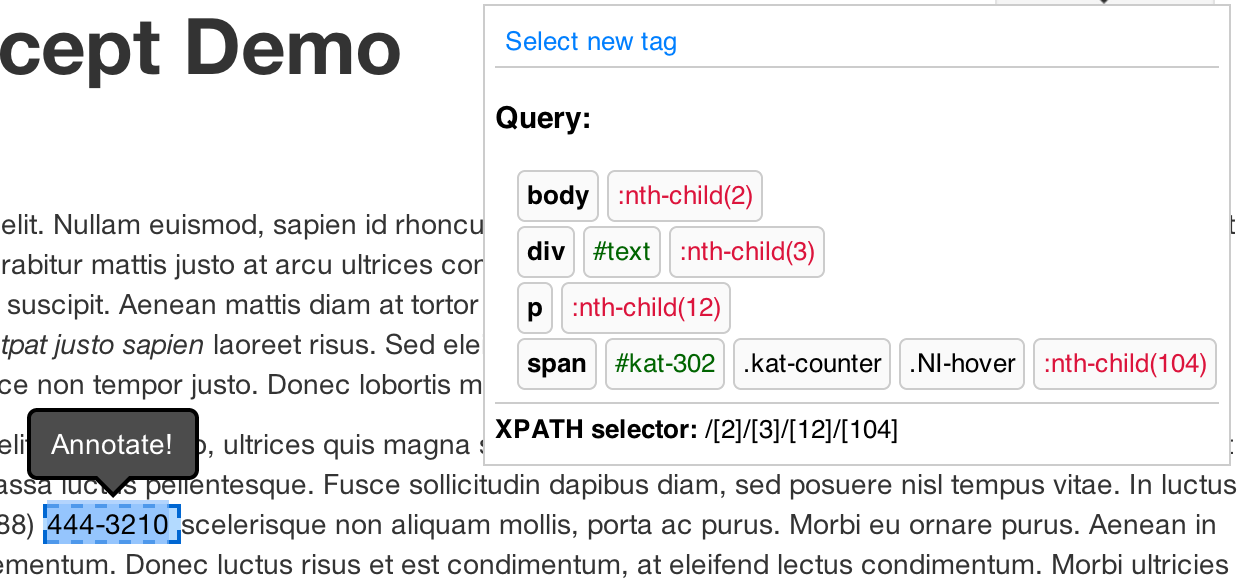
\includegraphics[width=5in]{../PIC/extension-annotate}
  \caption{Right-clicking on an element causes the "Annotation" pop-up to
    show}\label{fig:extension-annotate}
\end{figure}


%%% Local Variables:
%%% mode: latex
%%% TeX-master: "katmanual"
%%% End:

%  LocalWords:  includegraphics textwidth kat-annotate compactenum compactitem suscipit
%  LocalWords:  kat-definition ednote riew kat-review wrapfigure vspace katmanual

\section{Storage}

The annotation tool is storage agnostic per-se. As no back-end platform is provided
alongside the application, administrators are free to develop their own custom workflows
of storing an annotation. By default annotations are stored in the user's browser database
(or localStorage if the browser is older) and can be automatically transferred to a given
URI through a POST request. Annotations can also be loaded through GET requests from a
configurable URI or from the user's local storage.

Although the system is flexible in this regard, we recommend the storage of annotations in
a triple store as it provides a nicely continuity with the existing ontology based model.
The annotations can be easily represented as RDF structures and the application itself
stores it as so internally. Furthermore we believe that graph database are best suited for
storing and querying this kind of metadata.

\ednote{MK: Describe link to {Cor\TeX}~\cite{CorTeX:on,CorTeX:github:on}}

%%% Local Variables: 
%%% mode: latex
%%% TeX-master: "katmanual"
%%% End: 

\section{Conclusion}\label{sec:concl}
\ednote{MK: write something}
%%% Local Variables: 
%%% mode: latex
%%% TeX-master: "kat"
%%% End: 

\newpage
\printbibliography\newpage
\appendix
\section{Installation Guide}

In order to deploy \KAT, please follow the next steps:

\begin{enumerate}
\item In Makefile.in, change INSTALLDIR to the desired installation directory
  (e.g. /srv/http/kat or /var/www/kat).
\item Rename Makefile.in into Makefile. Run \textbf{make all \&\& make install}.
\item You will find a proof of concept demo at http://localhost/katInstallDir/test.
\item In order to add annotations, you need to add an annotation ontology first. You can
  do that in the \KAT Control Panel (link in the bottom-right of the page). For starting
  you can copy the example you find in test/annotations.xml.
\item The default storage environment is the browser's local storage. An API to connect to
  different storage environment can be found in the classes from the \textbf{remote/}
  directory.
\end{enumerate}

%%% Local Variables: 
%%% mode: latex
%%% TeX-master: "kat"
%%% End: 

\section{An Annotation Specification}
\ednote{MK: explain this and the features it corresponds to}
\lstinputlisting[language=XML,basicstyle=\footnotesize\sf]{ex/example-ontology.xml}

%%% Local Variables: 
%%% mode: latex
%%% TeX-master: "kat"
%%% End: 

%  LocalWords:  ednote lstinputlisting basicstyle footnotesize kat

\section{Developer Guide}
\KAT is written using FlancheJS: a simple library that provides javascript classical
inheritance. The classes are structured java-like, having:
\begin{itemize}
 \item constructors: provided by the method \textit{\textit{init}}.
 \item properties: the library automatically generates getters and setters.
 \item methods: publicly available functions.
 \item internals: properties and methods available only by underscore (\textbf{\textit{\_}}) prefixing.
\end{itemize}

The table below describes the \KAT classes (available under \textbf{src/js/}) and their behavior:

\begin{longtable}{p{6cm}|p{8cm}}%|
 \large{\textbf{Class Name}} & \large{\textbf{Class Description}}\\\hline
 \textbf{main} namespace: \\\hline
 \textit{kat.main.KATService} & The main entry point of the service. The \KAT Service requires a CSS3/XPATH selector to identify the container on which annotations can be made,
 and optionally a CorTeX service URL~\cite{CorTeX:github:on,CorTeX:on} and a document identifier for the annotated document.\\\hline
 \textbf{annotation} namespace: \\\hline
 \textit{kat.annotation.Annotation} & Describes an annotation that was collected from a user and can be saved and transported over
 network.\\\hline
 \textit{kat.annotation.AnnotationRegistry} & Describes an annotation registry that keeps track of all the annotations for the current document \\\hline
 \textit{kat.annotation.Concept} & Class to describe an annotation concept. Annotation concepts describe the annotation model (i.e. the fields contained
 by the annotation) and the behavior of the annotation (i.e. user interaction and display).\\\hline
 \textit{kat.annotation.ConceptRegistry} & A registry to keep track of all available concepts for this document.\\\hline
 \textit{kat.annotation.Ontology} & Class to describe an annotation ontology. Annotation ontologies describe the annotation concepts.\\\hline
 \textit{kat.annotation.OntologyRegistry} & A registry to keep track of all available ontologies for this document.\\\hline
 \textit{kat.annotation.AnnotationForm} & Class for handling the form displayed when an annotation is added.\\\hline
 \textbf{display} namespace: \\\hline
 \textit{kat.display.AnnotationEditForm} & Class for handling the form displayed when an annotation is edited.\\\hline
 \textit{kat.display.ControlPanel} & This class provides a tool for displaying and handling the \KAT Control Panel.\\\hline
 \textit{kat.display.AnnotationRenderer} & Class for handling the display of a singe annotation.\\\hline
 \textit{kat.display.ArrowConnector} &  Creates an svg arrow that can be used to connect two DOM elements, for example a reference field annotation to the referenced item.\\\hline
 \textit{kat.display.Display} & Creates and controls the annotation displays.\\\hline
 \large{\textbf{Class Name}} & \large{\textbf{Class Description}}\\\hline
 \textbf{input} namespace: \\\hline
 \textit{kat.input.Form} & The Form class decides which fields to be displayed in the current form. \\\hline
 \textit{kat.input.FormParser} & A form parser can be used to parse the fields and documentation from a given concept object.\\\hline
 \textit{kat.input.FieldParserRegistry} & The Field Parser Registry contains all the field parsers that are available to parse for a concept.\\\hline
 \textbf{input.fieldparser} namespace: \\\hline
 \textit{kat.input.fieldparser.FieldParser} & A field parser parses an annotation:field into an html string. This trait serves only as an interface that the extending classes follow. \\\hline
 \textit{kat.input.fieldparser.Checkboxes} & Parses a field of type checkboxes outputting html. \\\hline
 \textit{kat.input.fieldparser.Reference} & Parses a field of type reference outputting html. \\\hline
 \textit{kat.input.fieldparser.Select} & Parses a field of type select outputting html. \\\hline
 \textit{kat.input.fieldparser.TextArea} & Parses a field of type text area outputting html. \\\hline
 \textit{kat.input.fieldparser.TextField} & Parses a field of type text outputting html. \\\hline
 \textbf{input.fieldparser} namespace: \\\hline
 \textit{kat.input.view.Form} & Class that renders an annotation form containing the fields described in the concept. \\\hline
 \textit{kat.input.view.ConceptSelector} & Class to describe an input element in the form container that is used to select a concept to be used in the annotation form.\\\hline
 \textit{kat.input.view.FormContainer} & Describes a class that acts as a container for an annotation form and a concept selector.\\\hline
 \textbf{preprocessor} namespace: \\\hline
 \textit{kat.preprocessor.TextPreprocessor} & Used to add counters around text but this functionality has been deprecated. Now it only adds selection listeners in the text, for adding annotations.\\\hline
 \textbf{remote} namespace: \\\hline
 \textit{kat.remote.CoreTexAnnotationInserter} & Sends the annotations being created on this document to the CoreTeX system.\\\hline
 \textit{kat.remote.CoreTeXAnnotationReceiver} & Retrieves the document and the annotations from the CoreTeX service and populates the internal registry. \\\hline
\end{longtable}


%%% Local Variables: 
%%% mode: latex
%%% TeX-master: "kat"
%%% End: 

%  LocalWords:  FlancheJS textit textit textbf js longtable hline CorTeX svg kat
%  LocalWords:  input.fieldparser

\end{document}
%  LocalWords:  maketitle thispagestyle newpage tableofcontents includegraphics Yawas js
%  LocalWords:  vspace Annotatie Systeem interpretors textbf textit textit textit atleast
%  LocalWords:  atmost suscipit INSTALLDIR FlancheJS hline CorTeX svg input.fieldparser
%  LocalWords:  ednote soa datamodel printbibliography annospec
